\chapter{Proposal: PatientSPIRL}
\label{ch:proposal}

\section{Modeling in Healthcare}

\begin{figure}
  \centering
  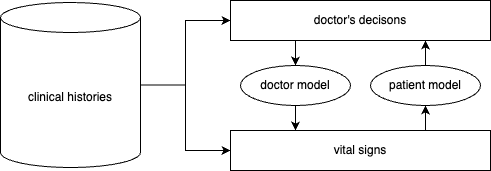
\includegraphics[width=0.8\linewidth]{images/PatientModeling.drawio.png}
  \caption{Modeling in Healthcare}
  \label{fig:modelhealth}
\end{figure}


\newpage
\section{Program Synthesis in Healthcare}

\todo{Make sure figures are connected to the text}

Healthcare is a domain where the advantages of program synthesis (as introduced in section \ref{sec:impacts}) are particularly relevant.
\begin{itemize}
    \item Inadequate \emph{capabilities} of decision systems in Healthcare present particularly challenging risks as patient's health and life can be at stake.
    \item No less dangerous is the risk of perverse incentives and insufficient \emph{alignment} of decision systems with the interests of the patient.
    \item Due to the risks above, Healthcare is a highly regulated domain and \emph{compliance by design} is a crucial feature of any decision systems deployed therein
    \item As a consequence, decision systems in Healthcare are never deployed fully autonomously. Instead, they have to support doctors in making the final decisions and have to be \emph{good team-players}, explaining the rationale behind every suggestion and supporting dialogue.
    \item \emph{Privacy} of clinical data is of utmost importance.
    \item Novel \emph{scientific discoveries} in healthcare have a particularly positive social impact.
\end{itemize}

This is especially relevant as healthcare systems struggle with understaffing \cite{ashleyy.metcalfHospitalUnitUnderstaffing2016,SurveyShowsHidden1993,UnderstaffingSignificantIssue2012,campbell_universal_2013, hudsonUnderstaffing2015, mercerMessageEditorinChief2008, r.stanleyUnderstaffedOverwhelmed2010, munnUnderstaffingWardsCompromising2017, thelancetHealthcareSystemStaffing2018}. Automation tools that make use of Machine Learning (also known as Healthcare 4.0 \cite{tortorellaHealthcareTrendsChallenges2020}) have been consistently identified as crucial for reducing the workload of Healthcare professionals and improving the quality of care \cite{agrawalMachineLearningHealthcare2020, deviDesignImplementationAdvanced2022, g.kumarSurveyMachineLearning2016, ganguliMachineLearningPursuit2020, maityMachineLearningImproved2017, mitraMachineLearningHealthcare2021, pianykhImprovingHealthcareOperations2020, xhaferraRoleMachineLearning2022}.


\begin{figure}
    \centering
    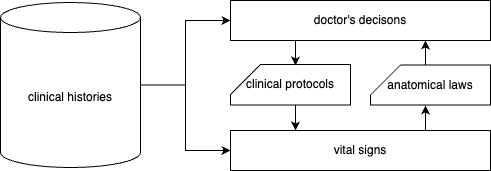
\includegraphics[width=0.8\linewidth]{images/PatientModelingInter.drawio.png}
    \caption{Interpretable Modeling in Healthcare}
    \label{fig:modelhealthinter}
\end{figure}



\newpage
\section{PatientSPIRL}

\begin{figure}
  \centering
  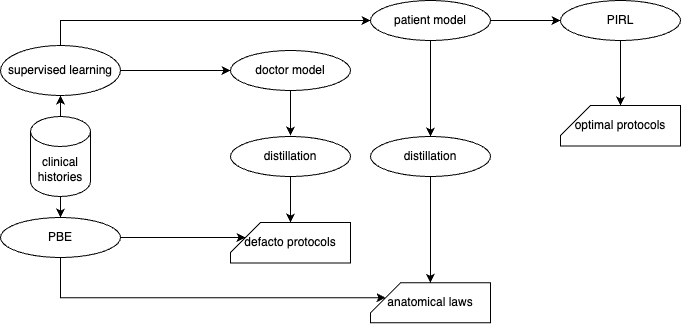
\includegraphics[width=\linewidth]{images/PSHealth.drawio.png}
  \caption{Patient Simulator Programmatically Interpretable Reinforcement Learning}
  \label{fig:pshealth}
\end{figure}
